\documentclass[a4paper,10pt]{article}
\usepackage{fullpage}
\usepackage{float}
\usepackage[english]{babel}
\usepackage{graphicx,subfig,wrapfig}
\usepackage{amsmath,amsfonts,amsthm,amssymb}
\usepackage{fancyhdr,fancybox,color}
\usepackage{enumerate}
\usepackage[amssymb]{SIunits}
\definecolor{MyBlue}{rgb}{0,0.3,0.6}
\usepackage[colorlinks=true,
linkcolor=MyBlue,
plainpages=false,
citecolor=MyBlue,
urlcolor=MyBlue]{hyperref}
\usepackage[all]{hypcap}
\usepackage[url=false,
backend=bibtex,
style=authoryear-comp,
doi=true,
isbn=true,
backref=false,
dashed=false,
maxcitenames=2,
maxbibnames=99,
natbib=true]{biblatex}
\DeclareNameAlias{author}{last-first}
\renewbibmacro{in:}{}
\addbibresource{refrence.bib}
\nonfrenchspacing
\begin{document}
\noindent Chair: Physics of Fluids group
\begin{center}
 \begin{LARGE}
 Sneeze droplets
   \end{LARGE}
\end{center}
\section*{Description}

During the COVID-19 pandemic, many of us wondered how viruses are transmitted from one person to another. It turns out that when we cough, sneeze, or speak, we produce numerous droplets that play a crucial role in spreading these viruses \citep{bourouiba2021fluid}. Understanding the final droplet distribution during such respiratory actions has been the aim of the scientific community ever since. 

From a physics perspective, coughing or sneezing can be understood as the airflow over a thin liquid layer attached to a surface \citep{kant2023bag}. This phenomenon is well understood for Newtonian fluids. However, this understanding does not apply well to human coughs, as the mucosalivary fluid exhibits non-Newtonian behavior. Consequently, we lack a comprehensive understanding of the influence of non-Newtonian effects on the overall dynamics. We have recently made efforts to understand the non-Newtonian effects of the breakup of jets (see \citet{dixit2024viscoelastic}).   

During the coughing, the breakup mucosalivary fluids into droplets take place in two steps. The first step is breaking liquid sheets into filaments, while the second step involves breaking those filaments into droplets. For Newtonian liquids, the overall dynamics are governed by a competition among three physical effects: capillarity, viscosity, and inertia \citep{anthony2019dynamics}. However, for mucosalivary fluids (which display viscoelastic properties),  elasticity also plays a crucial role\citep{sen2021retraction, liu2022contraction}. Understanding these dynamics, along with the resulting droplet size, is essential for analyzing sneeze droplets and developing effective strategies to mitigate airborne disease transmission.
You will numerically study the dynamics of the breakup of viscoelastic filament into the droplets (see figure \ref{fig:filament}). We will examine the overall dynamics and droplet size and compare our results with existing data on Newtonian fluids \citep{anthony2019dynamics}. Finally, the implication of our analysis will be made on the understanding of droplet distribution during coughing or sneezing. 


\begin{figure}[H]
\begin{center}
 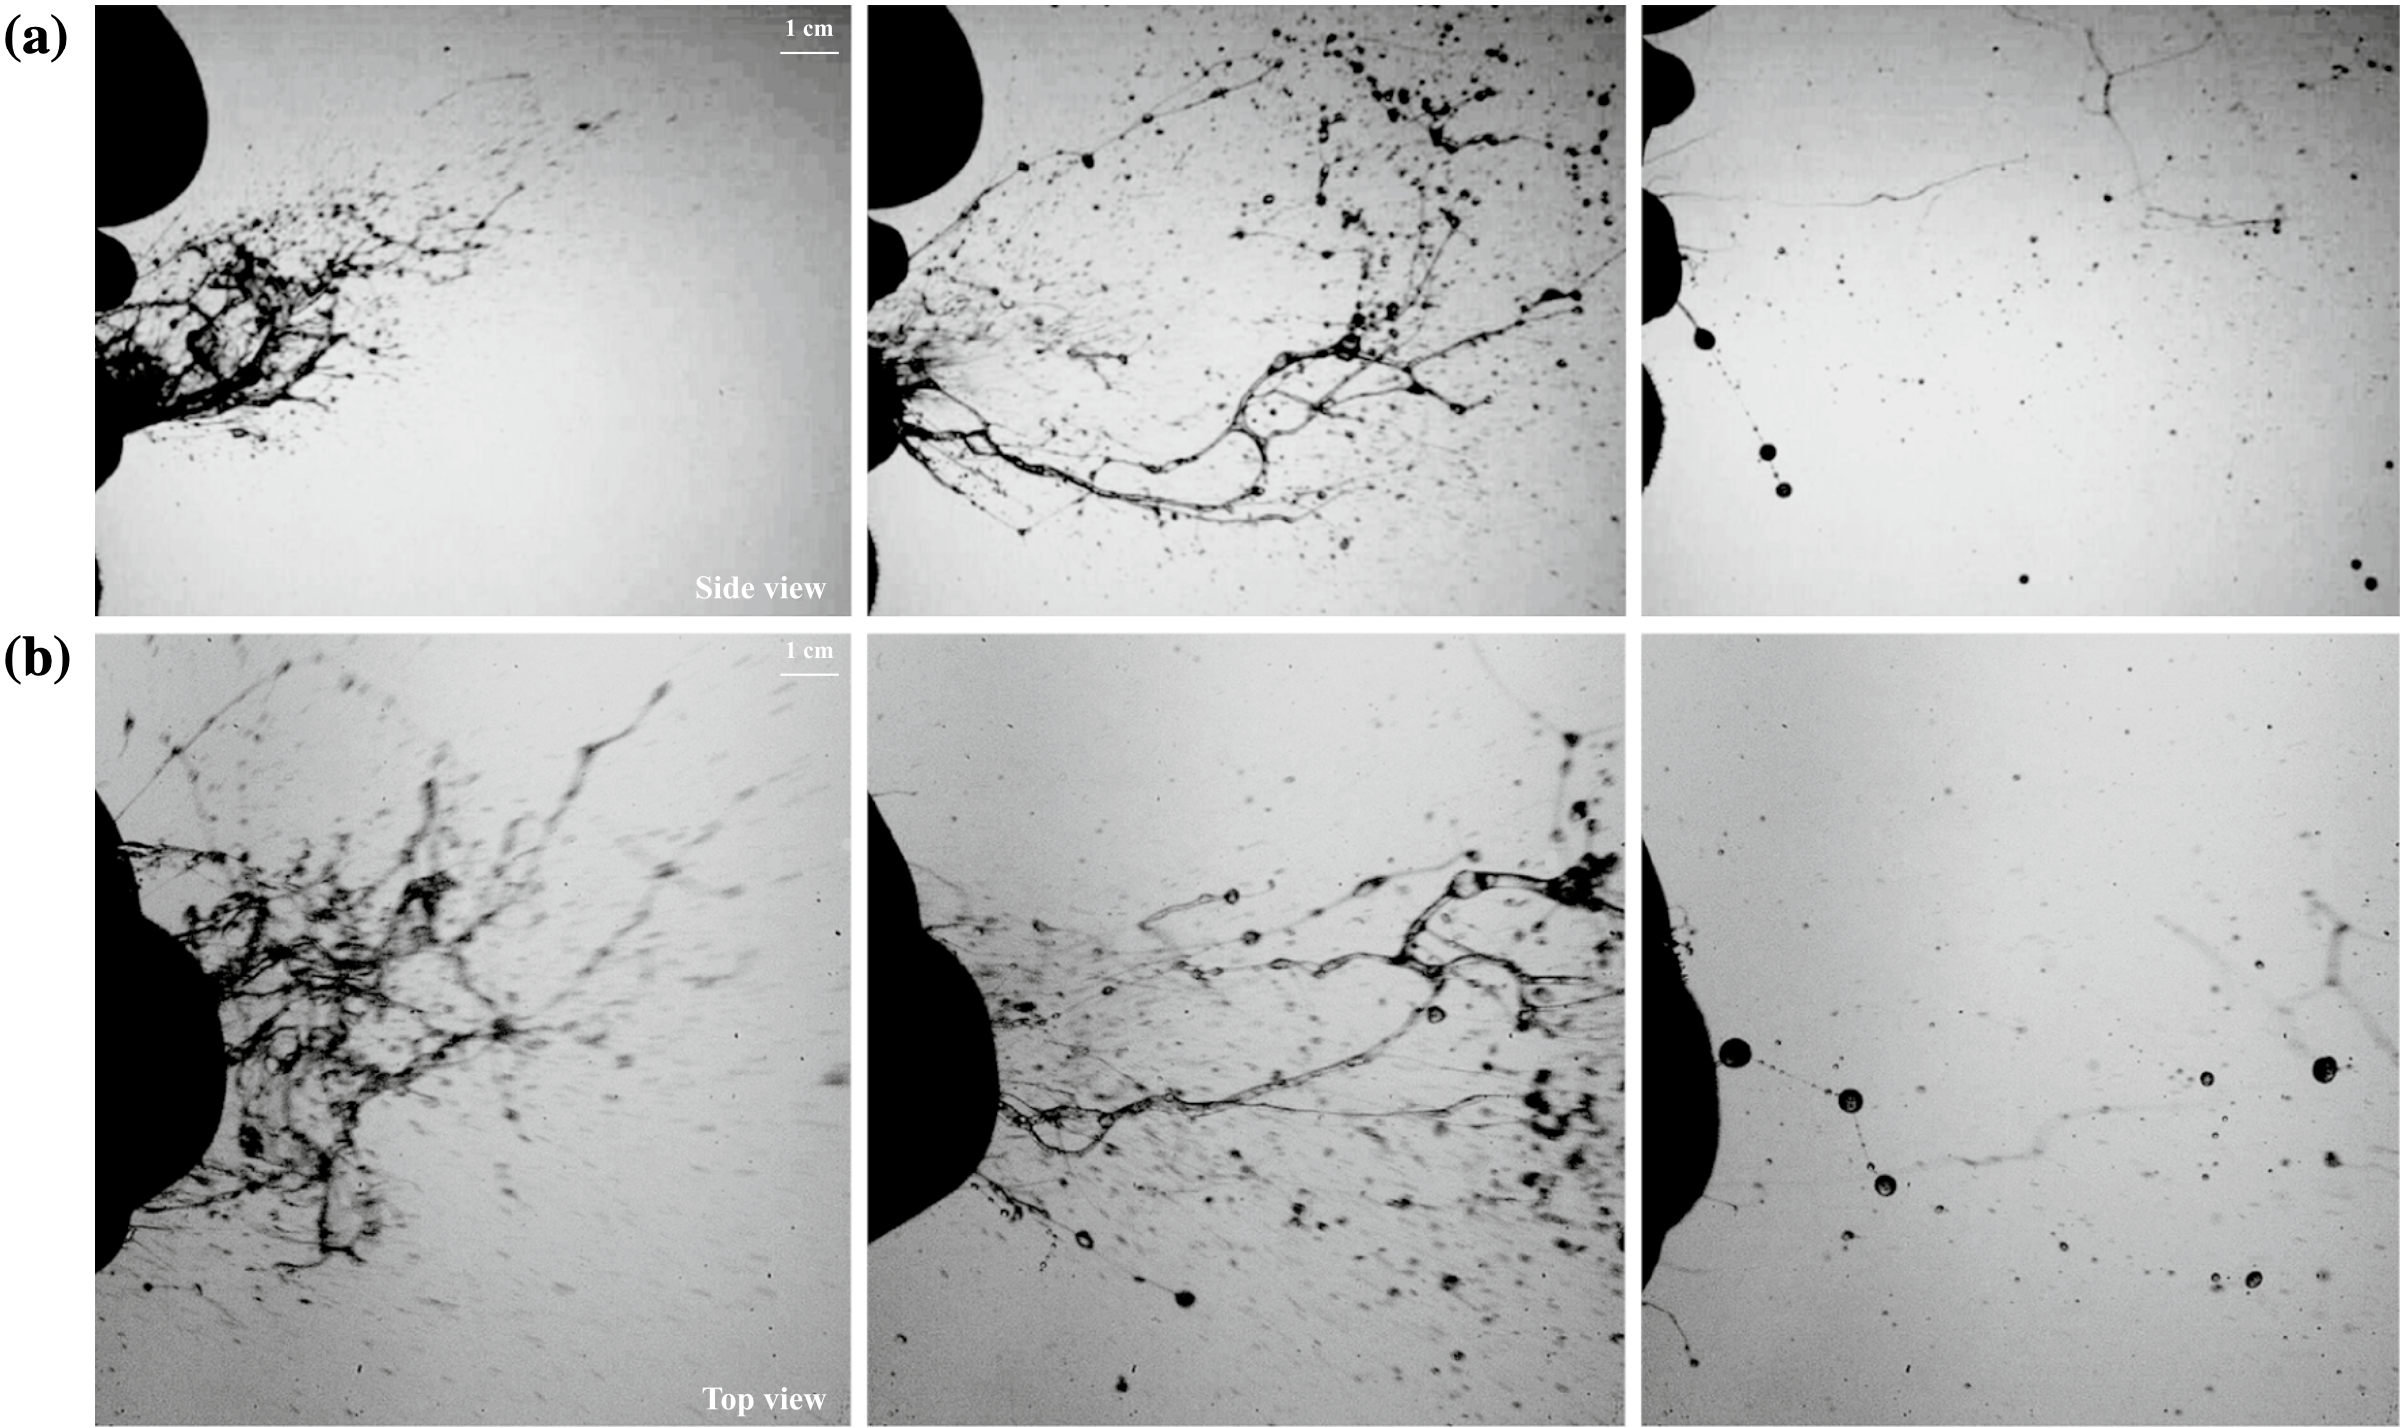
\includegraphics[width=0.95\textwidth]{sneeze.png}
 \caption{Stages of sneeze ejecta as experimentally reported by \citet{scharfman2016visualization}. One can notice several long filaments breaking up into droplets.}
 \label{Figure::Typical}
\end{center}
\end{figure}

\begin{figure}[H]
	\begin{center}
		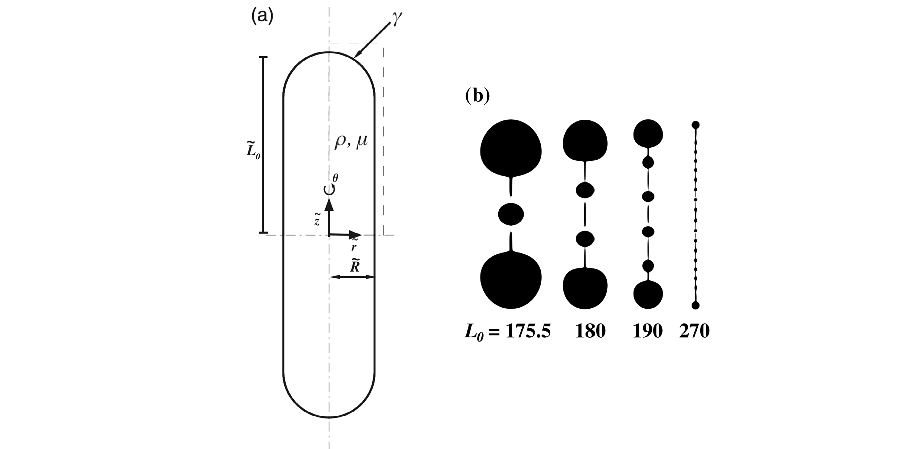
\includegraphics[width=0.75\textwidth]{filament_01.pdf}
		\caption{(a) Sketch of the initial filament, and (b) the final shapes obtained for different values of filament length $L_0$, studied for Newtonian fluids by \citet{anthony2019dynamics}. }
		\label{fig:filament}
	\end{center}
\end{figure}

\section*{What you will do and what you will learn?}
% The project will focus on the following:
\begin{enumerate}
\item You will learn about the physics of fluids, and science underlying non-Newtonian fluid flows. 
\item You will learn how to utilize computational tools to study real life physics. 
\item You will learn how to collaborate with a diverse group of researchers, specifically with other experimentalists and theoreticians.
\item You will have access to a read-to-use codebase (available on \href{https://github.com/comphy-lab/Viscoelastic-Worthington-jets-and-droplets-produced-by-bursting-bubbles}{GitHub}).
\item As a part of the \href{https://comphy-lab.org}{CoMPhy lab} at the Physics of Fluids Dept., you will learn and adapt open-source coding principles. 

\end{enumerate}

If you have any questions, feel free to contact \href{mailto:a.k.dixit@utwente.nl}{Ayush} (details below).
\begin{center}
\begin{tabular}{|l|l|l|}
\hline \textbf{Supervision} & \textbf{E-mail} & \textbf{Office} \\
\hline Ayush Dixit & \href{mailto:a.k.dixit@utwente.nl}{a.k.dixit@utwente.nl} & Meander 250 \\
\hline Dr. Vatsal Sanjay & \href{mailto:vatsalsy@comphy-lab.org}{vatsalsy@comphy-lab.org} & Meander 246B \\
\hline Prof. Dr. Detlef Lohse & \href{mailto:d.lohse@utwente.nl}{d.lohse@utwente.nl} & Meander 261  \\
\hline
\end{tabular}
\end{center}
\printbibliography
\end{document}
